% abtex2-modelo-trabalho-academico.tex, v-1.9.2 laurocesar
%% Copyright 2012-2014 by abnTeX2 group at http://abntex2.googlecode.com/
%%
%% This work may be distributed and/or modified under the
%% conditions of the LaTeX Project Public License, either version 1.3
%% of this license or (at your option) any later version.
%% The latest version of this license is in
%%   http://www.latex-project.org/lppl.txt
%% and version 1.3 or later is part of all distributions of LaTeX
%% version 2005/12/01 or later.
%%
%% This work has the LPPL maintenance status `maintained'.
%%
%% The Current Maintainer of this work is the abnTeX2 team, led
%% by Lauro César Araujo. Further information are available on
%% http://abntex2.googlecode.com/
%%
%% This work consists of the files abntex2-modelo-trabalho-academico.tex,
%% abntex2-modelo-include-comandos and abntex2-modelo-references.bib
%%

% ------------------------------------------------------------------------
% ------------------------------------------------------------------------
% abnTeX2: Modelo de Trabalho Academico (tese de doutorado, dissertacao de
% mestrado e trabalhos monograficos em geral) em conformidade com
% ABNT NBR 14724:2011: Informacao e documentacao - Trabalhos academicos -
% Apresentacao
% ------------------------------------------------------------------------
% ------------------------------------------------------------------------

\documentclass[
	% -- opções da classe memoir --
	12pt,				% tamanho da fonte
	openright,			% capítulos começam em pág ímpar (insere página vazia caso preciso)
	oneside,			% twoside, oneside - para impressão em verso e anverso. Oposto a oneside
	a4paper,			% tamanho do papel.
	% -- opções da classe abntex2 --
	%chapter=TITLE,		% títulos de capítulos convertidos em letras maiúsculas
	%section=TITLE,		% títulos de seções convertidos em letras maiúsculas
	%subsection=TITLE,	% títulos de subseções convertidos em letras maiúsculas
	%subsubsection=TITLE,% títulos de subsubseções convertidos em letras maiúsculas
	% -- opções do pacote babel --
	english,			% idioma adicional para hifenização
	brazil				% o último idioma é o principal do documento
	]{abntex2}

% ---
% Pacotes básicos
% ---
\usepackage{lmodern}			% Usa a fonte Latin Modern
\usepackage[T1]{fontenc}		% Selecao de codigos de fonte.
\usepackage[utf8]{inputenc}		% Codificacao do documento (conversão automática dos acentos)
\usepackage{lastpage}			% Usado pela Ficha catalográfica
\usepackage{indentfirst}		% Indenta o primeiro parágrafo de cada seção.
\usepackage{color}				% Controle das cores
\usepackage{graphicx}			% Inclusão de gráficos
\graphicspath{ {imagens/} }      % Local das imagens
\usepackage{microtype} 			% para melhorias de justificação

% Gráficos
\usepackage{pgfplots}
\pgfplotsset{width=10cm,compat=1.9}

% Para desenhar Flowcharts
% https://www.sharelatex.com/blog/2013/08/29/tikz-series-pt3.html
\usepackage{tikz}
\usetikzlibrary{shapes.geometric, arrows}
\tikzstyle{startstop} = [rectangle, rounded corners, minimum width=3cm, minimum height=1cm,text centered, draw=black, fill=red!30]
\tikzstyle{io} = [trapezium, trapezium left angle=70, trapezium right angle=110, minimum width=3cm, minimum height=1cm, text centered, draw=black, fill=blue!30]
\tikzstyle{process} = [rectangle, minimum width=3cm, minimum height=1cm, text centered, draw=black, fill=orange!30]
\tikzstyle{decision} = [diamond, minimum width=3cm, minimum height=1cm, text centered, draw=black, fill=green!30]
\tikzstyle{arrow} = [thick,->,>=stealth]

% http://www.texample.net/tikz/examples/pgf-umlsd/
\usepackage{pgf-umlsd}
\usepgflibrary{arrows} % for pgf-umlsd

% Formatação de código-fonte
\usepackage{listings}

% Altera o nome padrão do rótulo usado no comando \autoref{}
\renewcommand{\lstlistingname}{Código}

% Altera o rótulo a ser usando no elemento pré-textual "Lista de código"
\renewcommand{\lstlistlistingname}{Lista de códigos}

% Configura a ``Lista de Códigos'' conforme as regras da ABNT (para abnTeX2)
\begingroup\makeatletter
\let\newcounter\@gobble\let\setcounter\@gobbletwo
  \globaldefs\@ne \let\c@loldepth\@ne
  \newlistof{listings}{lol}{\lstlistlistingname}
  \newlistentry{lstlisting}{lol}{0}
\endgroup

\renewcommand{\cftlstlistingaftersnum}{\hfill--\hfill}

\let\oldlstlistoflistings\lstlistoflistings
\renewcommand{\lstlistoflistings}{%
   \begingroup%
   \let\oldnumberline\numberline%
   \renewcommand{\numberline}{\lstlistingname\space\oldnumberline}%
   \oldlstlistoflistings%
   \endgroup}


% ---
% Pacotes adicionais, usados apenas no âmbito do Modelo Canônico do abnteX2
% ---
% Pacotes de citações
% ---
\usepackage[brazilian,hyperpageref]{backref}	 % Paginas com as citações na bibl
\usepackage[alf]{abntex2cite}	% Citações padrão ABNT

% ---
% CONFIGURAÇÕES DE PACOTES
% ---

% ---
% Configurações do pacote backref
% Usado sem a opção hyperpageref de backref
\renewcommand{\backrefpagesname}{Citado na(s) página(s):~}
% Texto padrão antes do número das páginas
\renewcommand{\backref}{}
% Define os textos da citação
\renewcommand*{\backrefalt}[4]{
	\ifcase #1 %
		Nenhuma citação no texto.%
	\or
		Citado na página #2.%
	\else
		Citado #1 vezes nas páginas #2.%
	\fi}%
% ---

% ---
% Informações de dados para CAPA e FOLHA DE ROSTO
% ---
\titulo{Software de alta escalabilidade, performance e disponibilidade aplicada a reserva de ingressos online}
\autor{André Formento \and Danilo Hércules Araújo Sousa}
\local{Brasil}
\data{2017, v0.0.5}

\orientador{José Antônio Fonseca}
\instituicao{%
  Centro Universitário IBTA
  \par
  Engenharia da computação}
\tipotrabalho{Trabalho de conclusão de curso}
% O preambulo deve conter o tipo do trabalho, o objetivo,
% o nome da instituição e a área de concentração
\preambulo{Monografia apresentada ao Curso de Engenharia da Computação do Centro Universitário IBTA como parte dos requisitos para obtenção de Grau em Engenheiro da Computação.}
% ---


% ---
% Configurações de aparência do PDF final

% alterando o aspecto da cor azul
\definecolor{blue}{RGB}{41,5,195}

% informações do PDF
\makeatletter
\hypersetup{
     	%pagebackref=true,
		pdftitle={\@title},
		pdfauthor={\@author},
    	pdfsubject={\imprimirpreambulo},
	    pdfcreator={LaTeX with abnTeX2},
		pdfkeywords={abnt}{latex}{abntex}{abntex2}{trabalho acadêmico},
		colorlinks=true,       		% false: boxed links; true: colored links
    	linkcolor=blue,          	% color of internal links
    	citecolor=blue,        		% color of links to bibliography
    	filecolor=magenta,      		% color of file links
		urlcolor=blue,
		bookmarksdepth=4
}
\makeatother
% ---

% ---
% Espaçamentos entre linhas e parágrafos
% ---

% O tamanho do parágrafo é dado por:
\setlength{\parindent}{1.3cm}

% Controle do espaçamento entre um parágrafo e outro:
\setlength{\parskip}{0.2cm}  % tente também \onelineskip

% ---
% compila o indice
% ---
\makeindex
% ---

% ----
% Início do documento
% ----
\begin{document}

% Retira espaço extra obsoleto entre as frases.
\frenchspacing

% ----------------------------------------------------------
% ELEMENTOS PRÉ-TEXTUAIS
% ----------------------------------------------------------
% \pretextual

% ---
% Capa
% ---
\imprimircapa
% ---

% ---
% Folha de rosto
% (o * indica que haverá a ficha bibliográfica)
% ---
\imprimirfolhaderosto*
% ---

% ---
% Inserir folha de aprovação
% ---

% Isto é um exemplo de Folha de aprovação, elemento obrigatório da NBR
% 14724/2011 (seção 4.2.1.3). Você pode utilizar este modelo até a aprovação
% do trabalho. Após isso, substitua todo o conteúdo deste arquivo por uma
% imagem da página assinada pela banca com o comando abaixo:
%
% \includepdf{folhadeaprovacao_final.pdf}
%
\begin{folhadeaprovacao}

	\begin{center}
	{\ABNTEXchapterfont\large\imprimirautor}

	\vspace*{\fill}\vspace*{\fill}
	\begin{center}
		\ABNTEXchapterfont\bfseries\Large\imprimirtitulo
	\end{center}
	\vspace*{\fill}

	\hspace{.45\textwidth}
	\begin{minipage}{.5\textwidth}
		\imprimirpreambulo
	\end{minipage}%
	\vspace*{\fill}
	\end{center}

	Trabalho aprovado. \imprimirlocal, 20 de dezembro de 2017:

	\assinatura{\textbf{\imprimirorientador} \\ Orientador}
	% \assinatura{\textbf{Professor} \\ Convidado 1}
	% \assinatura{\textbf{Professor} \\ Convidado 2}

	\begin{center}
	\vspace*{0.5cm}
	{\large\imprimirlocal}
	\par
	{\large\imprimirdata}
	\vspace*{1cm}
	\end{center}

\end{folhadeaprovacao}
% ---

% Isto é um exemplo de Ficha Catalográfica, ou ``Dados internacionais de
% catalogação-na-publicação''. Você pode utilizar este modelo como referência.
% Porém, provavelmente a biblioteca da sua universidade lhe fornecerá um PDF
% com a ficha catalográfica definitiva após a defesa do trabalho. Quando estiver
% com o documento, salve-o como PDF no diretório do seu projeto e substitua todo
% o conteúdo de implementação deste arquivo pelo comando abaixo:
%
% \begin{fichacatalografica}
%     \includepdf{fig_ficha_catalografica.pdf}
% \end{fichacatalografica}
\begin{fichacatalografica}
	\vspace*{\fill}					% Posição vertical
	\hrule							% Linha horizontal
	\begin{center}					% Minipage Centralizado
	\begin{minipage}[c]{12.5cm}		% Largura

	\imprimirautor

	\hspace{0.5cm} \imprimirtitulo  / \imprimirautor. --
	\imprimirlocal, \imprimirdata-

	\hspace{0.5cm} \imprimirorientadorRotulo~\imprimirorientador\\

	\hspace{0.5cm}
	\parbox[t]{\textwidth}{\imprimirtipotrabalho~--~\imprimirinstituicao,
	\imprimirdata.}\\

	\hspace{0.5cm}
		1. Software
		2. Escalabilidade
		3. Performance
		4. Disponibilidade
		5. Microsserviço
		I. Orientador: \imprimirorientador.
		II. \imprimirinstituicao.
		III. \imprimirtitulo.\\

	\hspace{8.75cm} CDU 02:141:005.7\\

	\end{minipage}
	\end{center}
	\hrule
\end{fichacatalografica}
% ---

% isso aqui faz com que o sumário não quebre
% se remover ele gera -2 (menos 2) no número da página
\vspace{\onelineskip}


% resumo em português
\setlength{\absparsep}{18pt} % ajusta o espaçamento dos parágrafos do resumo
\begin{resumo}

  % https://blog.mettzer.com/resumo-abstract-tcc/

  Quando um sistema de ingressos abre as vendas para o público é comum
  que haja muita demanda, ou seja, um pico de requisições.
  Este trabalho apresenta uma abordagem com microsserviços para tratar
  especificamente do processo de reserva de ingressos.
  O objetivo é tornar a arquitetura elástica para que nesses momentos
  de grande demanda mais recursos fiquem disponíveis;
  e, quando a demanda for reduzida, haja otimização -
  garantindo assim escalabilidade, performance e disponibilidade.
  A conclusão mostra que a abordagem de microsserviços garantiu a
  abstração da camada de software, enquanto que a utilização de
  ferramentas adequadas permitiu a abstração da camada de hardware,
  e também, que toda a infraestrutura seja implantada em nuvem.
  Porém, as métricas mostraram que o serviço degradou-se ao receber muitas requisições.

  \textbf{Palavras-chaves}: Escalabilidade, Performance, Disponibilidade, Microsserviço

% escalabilidade
% performance
% disponibilidade
% microsserviço
% resultado
% balanceamento de cargas
% nuvem

\end{resumo}

% resumo em inglês
\begin{resumo}[Abstract]
 \begin{otherlanguage*}{english}
   When a ticket system opens the sales to the public is common
   that there is a lot of demand, that is, a peak of requisitions.
   This work presents a microservice approach to treat
   specifically the ticket reservation process.
   The goal is to make the architecture elastic so that in those moments
   demand more resources become available;
   and, when demand is reduced, there is optimization -
   ensuring scalability, performance and availability.
   The conclusion shows that the microservice approach has
   abstraction of the software layer, while the use of
   appropriate tools allowed the abstraction of the hardware layer,
   and also that the entire infrastructure be deployed in the cloud.
   However, the metrics showed that the service degraded upon receiving many requests.

   \vspace{\onelineskip}

   \noindent
   \textbf{Key-words}: Scalability, Performance, Availability, Microservice
 \end{otherlanguage*}
\end{resumo}


% lista de ilustrações
\pdfbookmark[0]{\listfigurename}{lof}
\listoffigures*
\cleardoublepage

% inserir lista de listings
% https://github.com/abntex/abntex2/wiki/HowToFormatarCodigoFonte
\pdfbookmark[0]{\lstlistlistingname}{lol}
\begin{KeepFromToc}
\lstlistoflistings
\end{KeepFromToc}
\cleardoublepage
% ---

\begin{siglas}
    \item[S\&P 500] Índice de mercado de ações composto por
                    quinhentas empresas diferentes conforme definido
                    por Kennon \cite{definicao-de-sp500}

    \item[Cliente web] É quem consome algum recurso da aplicação

    \item[JSON] JavaScript Object Notation ou Notação de Objetos JavaScript -
                é um formato legível para seres humandos e leve para ser trafegado \cite{define-json}

    \item[URL] Uniform Resource Locator ou Localizador Padrão de Recursos - é o formato de atribuição
               universal para designar um recurso na Internet \cite{define-url}
               
    \item[HTTP] O protocolo de transferência de hipertexto (HTTP) é um protocolo de camada de aplicação
               para transmissão de documentos hipermídia, como HTML. Ele foi projetado para comunicação
               entre navegadores e servidores web, mas também pode ser usado para outros fins \cite{define-http}
               
    \item[POST] Método HTTP. Na requisição HTTP em que é feita utilizando o método POST é possível enviar um anexo \cite{define-post}.
\end{siglas}


% sumario
\pdfbookmark[0]{\contentsname}{toc}
\tableofcontents*
\cleardoublepage

% ----------------------------------------------------------
% ELEMENTOS TEXTUAIS
% ----------------------------------------------------------
\textual

% regra de nome de arquivo:
% antes do _ está o nome da parte
% depois do _ está o nome do capítulo
% os nomes não devem ter espaços, caracteres especiais e devem ser separados por hífen

\part{Introdução}\label{introducao}
\chapter*[Introdução]{Introdução}
\addcontentsline{toc}{chapter}{Introdução}

Escrever introdução

\chapter{Organização}

O trabalho é divido em 4 partes:

\begin{itemize}
    \item \autoref{introducao} Introdução: nesta primeira parte é introduzido o que
          será tratado no trabalho, explicando o problema e deixando claros os objetivos;

    \item \autoref{conceitos} Conceitos: nesta parte são discutidos os fundamentos e
          argumentos para as tomadas de decisões de quais serão as melhores
          abordagens para resolver o problema;

    \item \autoref{implementacao} Implementação: nesta parte são explicadas as
          implementações do código fonte do serviço de reserva de ingressos, assim
          como, de como foi implementada e implantada a infraestrutura;

    \item \autoref{resultados} Resultados: nesta parte são exibidos os resultados
          práticos da implementação e conclusão das escolhas tomadas.

\end{itemize}

Todas as implementações mencionadas estão disponíveis através do link abaixo:

\url{https://github.com/andreformento/term-paper}

\chapter{Problema}

Atualmente a venda de ingressos para eventos ocorre em websites.
O comum é que haja muita divulgação na mídia a respeito do evento.
A venda de ingressos costuma ser muito disputada devido a limitação
física que o local onde ocorrerá permite, assim como, a oferta de
lugares privilegiados, ingressos com descontos (estudante, idoso), etc.
Desta forma, muitas pessoas buscam os ingressos logo após o início das
vendas, gerando uma demanda muito alta nas primeiras horas de venda.

Conforme \cite{10-motivos-para-vender-online}, os compradores consideram
vários motivos para fazer sua compra online, como comodidade por não
precisar ir até um ponto de venda; não enfretam fila; segurança; etc.

\index{alíneas}\index{subalíneas}\index{incisos}A venda de ingressos online
tem diversas temas a serem tratados. Porém, este documento abordará a parte
técnica do sistema focando nos seguintes itens que atenderá alta demanda:

\begin{alineas}

  \item Performance

  \begin{alineas}
     \item sites que não estão preparados para ter grande variação de tráfego
           tendem a ter problemas de performance ou lentidão
  \end{alineas}

  \item Escalabilidade

  \begin{alineas}
     \item vertical: aumento da capacidade computacional de cada equipamento.
           Há limitações físicas de escalabilidade e por isso não é aplicável
           para a solução final.
           Será abordado no trabalho somente a título de comparação.
     \item horizontal: aumento da quantidade de equipamentos
           (podendo manter o mesmo tipo de equipamento). Custo reduzido e
           disponibilidade escalável
     \item Motivação: possibilidade de distrubuição da execução da aplicação para satisfazer
           vários volumes de transação \cite{arquiteturas-em-n-camadas}
  \end{alineas}

  \item Disponibilidade

  \begin{alineas}
     \item quando não planejada, a alta demanda inesperada pode causar até mesmo
           indisponibilidade do sistema, fazendo com que fique temporariamente
           fora do ar;
     \item indisponibilidade causa perda de vendas. Segundo
           \cite{disponibilidade-downtime-perdas}, uma queda no serviço S3 da
           Amazon gerou um prejuízo estimado de \$160.000,00 somente nas empresas
           da S\&P 500
  \end{alineas}

\end{alineas}

\chapter{Objetivos}

\subsection{Objetivo Geral}

\subsection{Objetivos específicos}


\part{Conceitos}\label{conceitos}

\chapter{Conceitos de infraestrutura}

Para rodar um software é necessário que haja um hardware. De modo geral,
há duas estratégias de infraestrutura em que o hardware (servidor) antenderá a aplicação (software):
local (\autoref{infraestrutura-local}) ou em nuvem (\autoref{infraestrutura-em-nuvem}).

\begin{citacao}

Quando se trata de determinar a melhor forma de armazenar enormes quantidades de
dados empresariais confidenciais gerados diariamente, as organizações se deparam
com duas opções: (aquilo que pode ser considerado o método tradicional) sistemas
de armazenamento nas próprias instalações ou uma solução externa hospedada por
provedores de computação na nuvem. Embora muitas empresas continuem investindo
em armazenamento local, o armazenamento baseado na nuvem está começando a se
tornar uma opção potencial para algumas. De fato, espera-se que 36\% de todos
os dados sejam armazenados na nuvem até 2016, um crescimento da parcela de
apenas 7\% em 2013. Obviamente, apesar de o armazenamento em nuvem parecer
uma opção intrigante, existem pontos positivos e negativos associados a cada
método, desde custo e controle até segurança \cite{armazenamento-no-local-ou-na-nuvem}.

\end{citacao}

\section{Infraestrutura local}\label{infraestrutura-local}

Quando a insfraestrutura é local toda a responsabilidade é da empresa - manutenção,
compra de equipamentos e replicação do ambiente.
Ou seja, há necessidade atualizar software, comprar licenças de todos os programas,
fazer backup, garantir segurança física e lógica.
Todos os detalhes de como manter essa infra também são de responsabilidade da própria empresa -
como contratação de pessoas qualificadas e políticas de atualização.

Conforme \cite{beneficios-da-computacao-em-nuvem-para-sua-startup}, várias startups
tem optado por computação em nuvem por diversos motivos. Dentre eles, um que se destaca
em algo que pode ser muito relevante para a solução do problema da venda de ingressos, 
a escalablidade.

\begin{citacao}
Escalabilidade: Algo que é fundamental em qualquer startup é ser escalável.
Com infraestrutura em nuvem, sua empresa tem flexibilidade para aumentar e
diminuir os recursos conforme a demanda, sem a necessidade de comprar novos equipamentos, 
instalações de sistemas ou configurações complexas 
\cite{beneficios-da-computacao-em-nuvem-para-sua-startup}.

\end{citacao}

Em uma organização que possui uma variação muito grande da quantidade de demanda, lidar
com a escalablidade pode se tornar algo desastroso quando fala-se em custos. Imaginando
que a infraestrutura para atender a demanda da venda de ingressos estará limitada
pelos recursos de hardware que a organização terá, é possível imaginar que isso trará
vários problemas.

Por exemplo, Um cenário onde em um determinado horário a demanda por compra de ingressos 
esteja atingindo altos indices, a ponto de a infraestrutura alocada não suporte atender 
todas as requisições. Em um primerio momento, enxerga-se como solução a aquisição de mais 
equipemantos para suprir essa ineficiência. Porém, fora deste período de muitas vendas, essa
infraestrutura seria subutilizada. Em um caso pior, pode ser que haja mais de um evento que
tenham os ingressos com início das vendas no mesmo período. Desta forma, fica claro o problema
de tentar manter um infraestrutura própria para atender todas as demandas.

A ideia principal é que essa infraestrutura seja obtida de forma dinâmica. Por isso,
ter uma infraestrutura local, ou própria, é inviável para a solução do problema da
venda de ingressos.

\section{Infraestrutura em nuvem}\label{infraestrutura-em-nuvem}

Conforme \cite{what-is-cloud-computing}, computação em nuvem proporciona poder computacional
sob demanda através da internet. Desta forma, é possível que haja aumento de poder
de processamento conforme a necessidade do negócio - pagando apenas pelo que for utilizado.

\begin{citacao}
A computação em "nuvem", o chamado cloud computing, é um conceito que permite o acesso a
um conjunto de recursos como de processamento, armazenamento, conectividade, plataformas,
aplicações e serviços disponibilizados na Internet. Conjuntos de supercomputadores, que operam em
rede, formam a chamada "nuvem", que armazena softwares, documentos e aplicativos de um sistema.
Para ter acesso aos arquivos, basta que o usuário do cloud tenha acesso à internet
\cite{cloud-computing-conceitos-e-perspectivas-2012}.
\end{citacao}

Não é necessário grande investimento inicial para disponibilizar uma aplicação web.
Como o pagamento é pelo que for utilizado, se uma aplicação em determinado período tem
poucos acessos, então, pagará pouco; nos momentos onde há grande demanda, pagará por aquilo
que estiver utilizando. E é justamente essa flexibilidade que é fundamental para o sucesso
da solução proposta. Ou seja, toda a demanda de compra de ingressos poderá ser atendida
sem necessidade de investimentos em infraestrutura.

Conforme \cite{types-of-cloud-computing}, a computação em nuvem facilita a disponibilização
de aplicações aos desenvolvedores fazendo com quem foquem seu trabalho no desenvolvimento
do software.
Desta forma, ter toda a infraestrutura em nuvem é uma ótima escolha para lidar um sistema
de reserva de ingressos.

% pelo que vi tem mais artigos aqui: \url{https://canaltech.com.br/corporate/computacao-na-nuvem/}
% http://www.each.usp.br/dc/aulas/ComputacaoEmNuvem-DanielCordeiro.pdf

\subsection{Tipologia das plataformas em nuvem}\label{tipologia-das-plataformas-em-nuvem}

Com a popularização da computação em nuvem houve um aumento dos produtos e opções de
serviços disponíveis.
Desta forma, foram criados vários modelos e estratégias para utilização da computação
em nuvem, onde cada uma dessas estratégias foca em um determinado nível de abstração.
Há três principais formatos de nuvem que podem ser explorados:
IaaS (\autoref{iaas}), PaaS (\autoref{paas}) e SaaS (\autoref{saas}).
Recentamente vem surgindo um quarto formato que ainda é visto pelo mercado com
cautela: BaaS (\autoref{baas}).

% https://sistemas.eel.usp.br/docentes/arquivos/5840003/444/Cloudcomputing.pdf
% pagina 10

%\url{https://aws.amazon.com/pt/types-of-cloud-computing/}


\subsubsection{IaaS}\label{iaas}

No modelo Infrastructure as a Service (IaaS), ou Infra-estrutura como Serviço,
não há controle sobre o sistema operacional. O objetivo é o fornecimento
de recursos de computação necessários para rodar uma aplicação. Há acesso (virtual
ou hardware dedicado) em recursos de rede, computadores e acesso para armazenamento
de dados.
Um exemplo é o produto EC2 da Amazon.

%pode especificar cada uma delas:
%\url{https://apprenda.com/library/paas/iaas-paas-saas-explained-compared/}
%\url{https://antonioricardo.org/2013/03/28/o-que-e-saas-iaas-e-paas-em-cloud-computing-conceitos-basicos/}

\subsubsection{PaaS}\label{paas}

No modelo Plataform as a Service (PaaS), ou Plataforma como Serviço,
o foco é no gerenciamento da implantação e das aplicações.
Não há preocupação com aquisição de recursos, planejamento de capacidade,
manutenção de software, patching ou qualquer outro trabalho de baixo nível.
O Google AppEngine e a Amazon S3 são exemplos de PaaS.

\subsubsection{SaaS}\label{saas}

No modelo Software as a Service (SaaS), ou Software como Serviço,
há um produto completo, podendo ser oferecido inclusive como um aplicação
para o usuário final.
Aqui não há preocupações com serviço e nem gerenciamento de infraestrutura.
Um exemplo claro é o serviço de webmail, assim como Facebook,
Google Docs e Linkedin.

\subsubsection{BaaS}\label{baas}

Para esse modelo que é mais novo, há várias formas de definí-lo:
Backend as a Service (BaaS) ou Software como Serviço; Serverless Architectures; ou ainda,
Functions as a service (FaaS).
Nele fica abstraído inclusive a arquitetura de software da aplicação,
tendo como opção apenas desenvolver funções internas para execução. Desta forma, há grande
dependência da plataforma em que roda a aplicação.
Há vários serviços que podem ser facilmente consumidos como, serviço de chat, segurança com
OAuth, dentre outros.
Conforme \cite{martin-serverless}, há uma dependência também do ambiente em que roda o
código fonte, podendo inclusive necessitar de manutenção posterior em algo que está
funcionando pelo simples fato do fornecedor realizar alguma atualização.
Ou seja, há uma forte dependência com o fornecedor.

Alguns exemplos de BaaS são a AWS Lambda e Google Firebase.

\begin{citacao}
Um BaaS pode ser visto como uma ponte conectando o backend e o frontend de uma aplicação.
Os BaaS auxiliam os desenvolvedores a acelerar a criação de aplicações web e mobile e
simplificam a criação de APIs. Em vez de codificar o backend inteiro, o desenvolvedor usa
o BaaS para criar as APIs e conectá-las às aplicações \cite{backend-as-a-service-pros-e-contras}.
\end{citacao}

\subsubsection{Escolha da tipologia}

Cada tipologia discutida possui um nível de abstração que é proporcional ao nível de
dependência da plataforma, assim como, menor opção de customização para atender
o próprio negócio. Além do que, se for necessário um seriço específico, provavelmente
não existirá disponível. Como é o caso da reserva de ingressos.

Por isso, a escolha da tipologia foi de utilizar o modelo IaaS \autoref{iaas},
onde será possível instalar e escalar o serviço desenvolvido.
Essa infraestrutura em nuvem não foi implementada, mas da maneira como foi construído
e disponibilizado o serviço de reserva de ingressos, é possível usar qualquer modelo
de de IaaS disponível hoje no mercado, dependendo apenas de um sistema operacional
Linux.

% está é uma subsection de infraestrutura em nuvem do arquivo infraestrutura.tex

\subsection{Plataformas em nuvem}

Há diversas opções de plataformas em nuvem no mercado: AWS, Google Cloud Plataform,
Openstack Cloud, Microsoft Azure, Digital Ocean, etc. Dentre essas, há diferenças
de produtos oferecidos, preços, dentre outros fatores. Não será discutido aqui
especificidades de cada um.

Para o problema da reserva de ingressos, poderia ser usado, por exemplo, a AWS
que proporciona autoscaling \cite{aws-autoscaling} juntamente com o
Kubernetes \autoref{kubernetes}.
Desta forma, toda a infraestrutura seria escalável numa plataforma em nuvem
que hoje é considerada uma das maiores do mundo.

% \subsubsection{@AWS}
%
% Amazon Web Services (AWS)
%
% \url{https://aws.amazon.com/pt/}
%
% \url{https://aws.amazon.com/pt/blogs/compute/kubernetes-clusters-aws-kops/}
%
% \url{https://aws.amazon.com/pt/what-is-aws/}
%
% \url{https://aws.amazon.com/pt/about-aws/}
%
% tente focar no que ela pretende resolver (infraestrutura) e principalmente
% fazer links com o nosso tcc
%
% \subsubsubsection{@Auto Scaling na AWS}
% pode falar de produtos como Auto Scaling
% \url{https://aws.amazon.com/pt/autoscaling}
%
% e procura e me pergunta sobre outros assuntos relevantes pro tcc
%
%
%
% \subsubsection{@Google Cloud Platform (GCP)}
%
% nesse link também tem outros assuntos relacionados do lado direito
% \url{https://cloud.google.com/docs/overview/?hl=pt-br}
%
% você pode focar mais na AWS e não tanto no google plataform (se julgar necessario)
%
%
% \url{http://selbielabs.com/cloud-platforms-compared/}
%
% \subsubsection{@Heroku}
%
% \url{https://devcenter.heroku.com/}
%
% \subsubsection{@Digital Ocean}
%
% \subsubsection{@Microsoft Azure}
%



\chapter{Microserviços}\label{microservicos}

Como expressado por
\cite{building-microservices}, ``Microserviços são pequenos serviços
autônomos que trabalham em conjunto``.

\begin{citacao}
Em suma, o estilo arquitetônico do microserviço é uma abordagem para desenvolver
uma única aplicação como um conjunto de pequenos serviços, cada um executando em seu próprio processo e se comunicando
com mecanismos leves, muitas vezes uma API de recursos HTTP. Esses serviços são construídos em torno de recursos de
negócios e implementáveis independentemente por meio de maquinaria de implantação totalmente automatizada.
Existe um mínimo de gerenciamento centralizado desses serviços, que pode ser escrito em diferentes linguagens de
programação e usar diferentes tecnologias de armazenamento de dados \cite{martin-fowler-microservices}.
\end{citacao}

Com microserviços é possível escalar apenas algumas partes do sistema, diminuindo
o custo e esforço para aumentar o poder de processamento para atender muitas requisições.

Pode haver um serviço que cuida do contexto do usuário; outro serviço que lida com a
lista de eventos disponíveis; outro serviço responsável por realizar reserva de vaga de
cada evento; e assim por diante. Ou seja, cada um desses serviços pode ter a sua a quantidade
de requisições diferentes umas das outras, mas os serviços poderão ser escalados de forma
independente e conforme a necessidade.

Um exemplo real pode ser objservado em um e-commerce.

\begin{citacao}

Ao criarmos a Editora Casa do Código, decidimos seguir outro caminho para o e-commerce.
Lá não podemos correr o risco de ficar com a loja fora do ar caso alguma funcionalidade
periférica falhe, então quebramos nossa arquitetura em serviços menores. Dessa forma, há
um sistema principal, que é a loja e está hospedada no Shopify, e vários outros sistemas
que gravitam em torno dela. Temos uma aplicação que faz a liberação dos e-books para os
clientes, outro que contabiliza os royalties para autores, outro para cuidar da logística
de envio dos livros impressos para o cliente, um painel de visualização dos livros comprados,
um para fazer a liberação de vale presentes e outro para promoções.

Dessa forma, quando um evento acontece na nossa loja online, os diferentes sistemas precisam
ser notificados. Para essas notificações usamos requisições HTTP, assim, quando uma compra
é confirmada na loja online, todos os sistemas recebem em um Endpoint essa requisição HTTP,
contendo um JSON com todos os dados da compra. Cada sistema decide o que fazer com as informações
recebidas, de acordo com a necessidade. Por exemplo, o sistema de liberação dos e-books verifica
se a compra possuía e-books e gera os links de download para o comprador, enquanto que o sistema
de logística já dá baixa no estoque quando a compra é de um impresso, além de notificar as pessoas
quando algum livro está ficando com estoque crítico. Essa característica importante para o maior
desacoplamento dos serviços é conhecida como Smart endpoints, dumb pipes, que em uma tradução
livre pode ser entendida como Endpoints inteligentes e fluxos
simples \cite{arquitetura-de-microservicos-ou-monolitica}.

\end{citacao}


Considerando que a reserva de ingressos é um contexto bem definido, pode haver um serviço que cuide
especificamente desta parte. Desta forma, é possível isolar e pensar de forma objetiva em como
lidar com esse problema.

\section{Comparação entre microserviços e sistemas monolíticos}\label{microservicos-monoliticos}
A implementação de microseviços deve-se ao fato de resolver problemas na estrutura do sistema. Com o aumento exponencial
na quantidade de aplicações que são desenvolvidas, tem-se milhares de bases de códigos. Essas bases
aumentam tanto de tamanho como de complexidade, características dificultam a equipe de desenvolvimento, ao passo que a
medida que o código cresce, torna-se difícil reparar ou realizar mudanças. Esse cenário torna-se mais desafiador quando
fala-se de um sistema monolítico. Para que se entenda as vantagens de usar os microserviços, pode-se comparar a arquitetura
monolítica.


Um programa monolítico é estruturado usando desvios condicionais ou incondicionais, não fazendo uso explicito de mecanismos
auxiliares de programação que permitam uma melhor estruturação do
controle \cite{teoria-da-computacao-3ed-ufrgs-maquinas-universais-e-computabilidade}.


Nos microserviços a independência de sua implantação é algo tido como uma das razões para utilizá-los ao invés das
bibliotecas. Estas são atreladas a um único processo, mesmo contendo várias bibliotecas, todas estarão atreladas ao mesmo
processo, uma vez que se faz alterações em qualquer delas, resulta em uma implantação do aplicativo inteiro.
As vantagens em microserviços abrangem desde a equipe atuante no desenvolvimento, já que com nesse paradigma, elas planejam
uma atuação em serviços diferentes, sem que essas mudanças afetem os demais integrantes. Adere a escalabilidade de forma
seletiva, possibilitando escalar somente a parte do sistema que necessita de ajustes. A divisão do sistema também beneficia
a velocidade de desenvolvimento, o código tratado é de fácil entendimento e como são soluções relativamente pequenas
compilam mais rápido. Huy Hutnh e Magnus Bjorkman, arquitetos da Amazon AWS em um artigo mencionam em sua conclusão as práticas relatadas.

\begin{citacao}
A migração de um aplicativo monolítico para um conjunto de microserviços em contêiner pode parecer uma tarefa assustadora.
Seguindo as etapas assertivamente, você pode começar a contornar aplicativos monolíticos, aproveitando o ambiente de tempo
de execução do contêiner e iniciando o processo de reestruturação em microservices. No geral, os microservices em
contentores são mais rápidos de desenvolver, mais fáceis de iterar e mais económicos para manter e
proteger \cite{deploying-java-microservices-on-amazon-ec2-container-service}.
\end{citacao}

\chapter{Escalabilidade}\label{escalabilidade}


Escalabilidade é uns dos pontos centrais que o trabalho propoem, isso porque a alta escalabilidade esta
atrelada a capacidade de um sistema conseguir se adequar a qualquer nivel de processamento e solicitação
que nele for imposto. Esse tema abordará a escalabilidade de forma conceitual e como ela pode ser implementada.


\begin{citacao}

À medida que o volume de dados cresce, aumenta a
necessidade de escalabilidade e melhoria de desempenho. Dentre as soluções para este
problema, pode-se citar a escalabilidade vertical, que consiste em aumentar o poder de
processamento e armazenamento das máquinas, e a escalabilidade horizontal, onde ocorre um
aumento no número de máquinas disponíveis para o armazenamento e processamento de
dados. Em comparação com a escalabilidade vertical, a escalabilidade horizontal tende a ser
uma solução mais viável, porém requer que diversas threads/processos de uma tarefa sejam
criadas e distribuídas. \cite[3]{alexandre-morais-souza-2013}.

\end{citacao}


O trabalho sugere uma possivel solução para o problema de queda de serviços quando estes são 
sujeitos a uma quantidade muita alta de requisições. A inatividade desses serviços resulta em perda 
de acessos, requisições sem respostas ou tempo de espera expirado.A forma 
como contorna-los serão tratadas nesse capitulo. 


A escalabilidade horizontal é preferível por diversos fatores - principalmente por
permitir que seja possível ampliar a capacidade de processamento de requisições
apenas aumentando a quantidade de nós (unidades de processamento/computadores).
Além do que, dada uma arquitetura preparada, é possível fazer a automação da
arquitetura para que permita que novos nós sejam adicionadas enquanto o
sistema está recebendo requisições, tornando possível que aumente a capacidade
de processamento \cite{ivens-oliveira-porto-2009}.

Quando há um aumento significativo de processamento, memória, threads, etc,
é possível que novas máquinas sejam incluídas como nós de processamentos.
Isso é possível devido ao monitoramento das máquinas existentes na arquitetura
da aplicação.

Por exemplo, um parâmetro de máximo de processamento de 80\% é configurado.
Quando a aplicação atingir esse parâmetro, outro nó poderá ser iniciado para ajudar
a atender as demandas do sistema. Da mesma forma, pode ser configurada uma utilização
mínima. Por exemplo, quando o processamento chegar à 20\% de utilização, uma máquina
deve ser finalizada, economizando custos de infraestrutura.




%%%%%%%%%%%%%%%%%%%%%%%%%%%%

% daqui pra baixo são apenas comentários que fiz:

% \url{https://github.com/lhzsantana/escalabilidade}
%
% \section{Apache Kakfa}
% Apache Kakfa, para queueing
% \url{https://medium.com/@gabrielqueiroz/o-que-%C3%A9-esse-tal-de-apache-kafka-a8f447cac028}
%
% \section{Apache Spark}
% Apache Spark, para streaming
% \url{https://www.infoq.com/br/presentations/spark-streaming-kafka-sem-perdas}
%
% \section{Apache Cassandra}
% Apache Cassandra, para registro de transações

% vou ver exatamente como escrever sobre os seguintes assuntos:
%
% java usando técnicas de imutabilidade
% Rest para requisições síncronas
% Kafka para gerenciar fila de processamento (garantir ordem)
% Websocket para receber notificações (mosquitto


\chapter{Disponibilidade}

Alta disponibilidade

Muito utilizado em tecnologia, alta disponibilidade é descrita como a maneira de identificar, corrigir e evitar falhas ao longo do tempo de operação do sistema. Visa atender o máximo de tempo possível as requisições solicitadas. Para que isso seja alcançado, é necessária uma infraestrutura complexa, uma redundância nos equipamentos físicos e uma orquestração de plataformas que devem estar em harmônia com o hardware. Sistema que gerenciam esse conjunto de equipamentos são desenvolvidos de maneira específica, eles são adequados para que consigam usar todos os recursos que o hardware possa oferecer. Normalmente o software é construído em paralelo com o hardware, porém atribuindo ao kernel configurações existentes que compõem os equipamentos. Caso haja alguma anomalia ou falhas que comprometam o sistema, este é capaz de abortar sessões onde estão ocorrendo os problemas e disponibilizar outro ambiente livre que atenda o operador, ou seja, a interrupção muitas vezes não impactam os processos existentes.
Toda essa complexidade resulta em um sistema que opera muitas vezes em mais de 95% do tempo. Esse período é medido anualmente, para conhecer o tempo de inatividade do componente utiliza-se uma fórmula, esta possui como parâmetros, graus de tolerância e tempo médio entre falhas. Os cálculos são feitos com a equação abaixo;
MTBF- Mean Time Between Failures - (tempo médio entre falhas)
MTTR- Mean Time To ReMpair - (tempo médio de recuperação)
Disponibilidade = MTBF / (MTBF + MTTR)
Um sistema que garante 99% do tempo anualmente tolera até 3,65 dias por ano de inatividade. Números atrativos para muitas empresas, porém organizações que atuam na internet exigem um tempo disponível mais alto do que o exemplificado. Organizações que trabalham com serviços web, priorizam o máximo do tempo on-line e buscam serviços que entregam o menor tempo de inatividade possível. Para atender essa necessidade, empresas investem em maquinários e infraestrutura que tem um custo elevado, mais desempenham um alto grau de operação, atingindo 99,999% do tempo de atividade por ano, um downtime/ano de apenas 5 horas.
Empresas que possuem negócios on-line, são as que mais requisitam esse serviço. Reduzir eventos como falhas e interrupções agregam mais confiança e fidelidade dos clientes, por esta razão, muitos negócios estão sendo migrados para essa plataforma. Fora do âmbito tecnológico, outras empresas estão se tornando cada vez mais globalizadas. Essas mudanças implicam novos desafios, um deles é a criticidade de acessar as informações em onde quer que estejam. Visto que isso é uma demanda crescente a alta disponibilidade está é uma alternativa que atende qualquer ramo de negócio, seja ele pequeno, médio ou de grande porte.
Com as diversas vantagens apresentadas, a alta disponibilidade tem seu preço. Os benefícios podem ser aproveitados, porém estão atrelados pela necessidade ainda maior de um hardware robusto que consiga absorver milhões de requisições por segundo. Essas requisições são oriundas de todas as partes do planeta e precisam ser atendidas no menor tempo disponível. Constantes indisponibilidades em aplicações que são críticas, causam perdas de clientes ou tarefas e a imagem negativa que é associada a empresa torna-se duradoura e difícil de apagar.
Algumas terminologias usadas em alta disponibilidade são as mesmas que se usa em computação, com algumas mudanças. O sistema que se usa em alta disponibilidade pode ser o resultado de um conjunto de subsistemas que são capazes de executar funções individuais, porém sua principal utilidade é integrar e auxiliar os demais subsistemas que garantem uma operação única, um comportamento similar aos sistemas que se utiliza em ou pequenas ou médias empresas, mais são compostos de apenas um sistema que gerencia todos os componentes e demais softwares.
O sistema operacional que atua em alta disponibilidade, é projetado para além de outras funções, monitorar o hardware, a fim de tomar decisões que redirecione as requisições, caso intercepte falhas que comprometam a execução da tarefa. Esse monitoramento é um dos pilares que garantem e classificam um sistema altamente disponível.
O sistema oferece aos seus utilizadores serviços. Estes são disponibilizados e executam uma série de instruções requisitadas pelo operador.
Apesar de trabalhar com o intuito principal de evitá-las, esses sistemas ainda estão passiveis de falhas. Repostas não esperadas, interrupções físicas, eventos inesperados que podem estar no hardware e afetam o funcionamento interferindo na disponibilidade. Cada ocorrência que não esta dentro do que é esperado é classificada como falha. Apesar de não esperada, ela deve ser corrigida com o menor tempo possível. Sua origem esta relacionada com falhas humanas ou não, esses eventos incorretos depois de corrigidos passam a ser tratados de forma a evitar-se no futuro. Depois de armazenar essas falhas, elabora-se relatórios que apontam o tempo médio de falhas existentes. Todo hardware está fadado ao envelhecimento, o tempo médio de falhas aponta o quanto esse sistema está passível de quedas, analistas utilizam esses resultados para manutenção preventiva ou na aquisição de novos componentes.
Existe também outro tempo mensurado para conhecer-se as discrepâncias do sistema. Somando-se todas as diferenças entre tempo desligado e o tempo ligado, dividindo pelo número de falhas obtidos anteriormente, consegue-se obter o tempo médio entre falhas. Utiliza-se esse tempo para se ter uma previsão do tempo de atividade do sistema em sua vida útil. Essa previsão faz parte de uma análise que conseguirá avaliar casos que reparação ou até mesmo renovação do conjunto.
As falhas que exitem podem ter sua origem a partir de um defeito. Utiliza-se o termo defeito quando o sistema apresenta resultados inesperados dentro de uma análise realizada pelo usuário. Trava-se a imagem, exibe-se dados incorretos ou mensagens erros, maneiras que o conjunto usa para alertar o usuário que algo esta errado. Certas situações não são percebidas de imediato, estas permanecem nos sistemas causando latências e inatividade.
O estado errôneo ou em erro, pode ser percebido quando se tem no processamento posterior um defeito. Este estado está relacionado em um universo informacional. Decorrente de uma falha o sistema apresenta informações incoerentes ao resultado esperado. O comportamento não atende as exigências de um funcionamento adequado causando-se defeitos que serão observados pelo operador. Entende-se que a classificação dos estados citados são estados de falha, que abrange toda parte física, estado de erro o que compete ao universo informacional e o estado de defeito que está relacionado em um cenário controlado pelo usuário.
De tal relevância no assunto, as falhas foram ao logo de tempo muito estudadas, concluiu-se que dentro do estado de falha é possível identificar tipos diferentes desse comportamento.
Distingue-se as falhas por duração como transientes ou permanentes. A primeira possui tempo de duração curto, suas causas estão atreladas ao mal funcionamento ou alguma interferência externa indesejada. Elas também podem ser intermitentes, afetando a operação em curtos porém diversos momentos distintos.
Falhas que causam problemas de forma a não operar todo o hardware com consistência,
 eventos afetam de tal maneira que o desempenho é comprometido permanentemente, conhecidas como falhas permanentes, estas impossibilitam o sistema a funcionar como antes do ocorrido.
Passível de outras falhas que competem a algum componente específico, conhece-se essas falhas como;
De travamento, bem intuitivo esta falha representa algum travamento causado por um componente que apresenta defeito e perde-se do seu estado interno normal.
Quando um componente responde requisições que a ele foram solicitadas, de forma antecipada ou atrasada, ele está fora de sincronismo com os demais, chama-se esse evento de falhas de timing ou falhas de performance.
Falhas por omissão se dão por conta de um processo que ao entrar em colapso não conseguiu executar o próximo passo do programa. A não execução foi repentina, ou seja, quando foi invocado o processo ele simplesmente não respondeu. Outros processos identificam a falha por omissão através de timeouts, as requisições possuem tempo de espera, caso esse período seja ultrapassado, considera-se esse estado com falha.
Caso o sistema opere de forma assíncrona, esta falha pode ser tratada como uma reposta ainda não recebida ou lenta. Para que o colapso da falha possa ser identificado, outros processos precisam detectar essa ocorrência, considerando o timeout de cada processo envolvido. Diferente do anterior, o sistema síncrono tem por sua vez os períodos idênticos de reposta de cada processo, caso não responde nesse tempo preestabelecido, concluiu-se falha na execução.
Outro ponto a ser abordado no que se refere a falhas por omissão, são as falhas por comunicação. Considere-se os princípios simples de comunicação, o envio e recebimento de mensagens também possuem falhas. O fluxo inicia-se enviando uma mensagem, está é armazenada no buffer do recebedor. Quando o processo identifica que o buffer possui novas entradas, recupera essa mensagem. Quando ele não se concretiza por completo, o canal de comunicação determina falha de omissão por comunicação.
Falhas arbitrárias ou bizantinas – avalia-se como uma das piores situações de falhas dentro do sistema. Isso porque é de difícil detecção, já que seus sintomas não são visíveis tão facilmente. Nesse estado, pode-se assumir valores diferentes dos seus dados, retornando um resultado errado mesmo que as vezes próximo do esperado. Noutro exemplo, falhas arbitrarias podem surgir afetando os canais de comunicação com mensagens corrompida ou inconsistentes.

\chapter{Balanceador de carga}

Balanceamento de carga é uma técnica que tem por objetivo a distribuição de carga de trabalho uniformemente entre dois ou
mais computadores. Essa técnica também pode ser utilizada em enlaces de redes e discos rígidos. O mecanismo visa atingir
escalabilidade do sistema e propiciar alta disponibilidade de acesso e respostas de requisições, ou seja, a medida que a
demanda pelos serviços, recursos ou o número de usuários conectados aumentam, mais máquinas são acionadas para incorporar
o conjunto e auxiliar no processamento dos dados.


O balanceamento de rede, consiste na técnica de distribuição de tráfego de rede entre servidores. Essa solução visa entregar
caminhos alternativos a fim de descongestionar os acessos atendendo um número maior de requisições. A segunda geração dos
balanceadores de carga são seguidos pelos sistemas proprietários baseados em aplicativos. Se comportam de forma transparente
as aplicações, ou seja, quando um único servidor não comporta toda carga gerada, é possível iniciar uma nova instância em
outro servidor e balancear a aplicação entre eles.


Utilizando-se do balanceamento de carga, o trabalho propõem tratar um problema que está relacionado com a exponencial
quantidade de requisições recebidas pelos servidores que hospedam sites de vendas de ingresso. A sobrecarga de um
sistema pode ocorrer de maneira linear - com o passar dos anos, por exemplo; ou ainda, exponencial - algum pico de uso
que pode ocorrer com o rápido aumento de requisições em questão de minutos.
No caso do problema da reserva de ingressos, esses picos podem ocorrer regularmente a cada abertura da venda de ingressos.
Com estes pico, cada vez que houver aumento de processamento das requisições e os servidores passarem a entrarem em
estado de sobrecarga, mais servidores podem ser disponibilizados para atenderem a alta demanda e o balanceador de carga
ficaria responsável por distribuir a carga para esses novos servidores também, tornando assim a estrutura escalável
horizontalmente.

O problema poderia demandar uma série de outros problemas para o provedor, isso porque este perderia uma quantidade muita
alta de clientes, muitos desistiriam ou iriam adquirir o produto de outra forma. A confiabilidade da empresa web seria
abalada negativamente, pois diante da frustração, os usuários poderiam passar uma imagem inadequada e que implicaria a perda
de possíveis novos clientes. Consumidores de produtos que compram pela internet, possuem um comportamento que difere em
alguns casos dos compradores de lojas físicas. Eles estão acostumados com um atendimento simples, rápido e sem burocracia.
Quando desejam adquirir algo, seus possíveis vendedores devem oferecer uma experiência que abrange tudo que ele irá
necessitar para comprar o produto, alguma inatividade no site pode significar a perda de uma venda.


Ao que compete a empresa contratante, o provedor do serviço, também sofreria e sua imagem como empresa confiável seria
duramente criticada. A razão pelo efeito dominó está que a única forma de colocar os produtos acessíveis ao público é de
forma virtual. Inconsistências no acesso dos clientes podem ser comparados as portas fechadas de uma loja física.


Sugere-se como uma solução que atende as exigências citadas a utilização de balanceamento de carga baseado em hardware.
Essa tecnologia tem por base dispositivos de rede. Esses diapositivos são neutros em relação aos aplicativos, dessa forma
consegue-se atuar em qualquer plataforma. Em resumo, os componentes oferecem um “servidor virtual” para todos os serviços
que requerem acesso, quando o servidor aceita a requisição, encaminha a mesma para o “servidor real” disponível para atender
e processar os dados. Suas vantagens frente aos demais, é o controle dos servidores, sua disponibilidade, atividade e
operação, monitorado do estado do hardware, isso garante que o sistema irá responder todas as requisições sem perder
desempenho. Com esse gerenciamento também é possível detectar quando os servidores recebem baixo número de acessos, nesse
estado algumas máquinas são desativadas temporariamente, visando economia de energia e preservação dos equipamentos.



\part{Implementação}\label{implementacao}

\chapter{Arquitetura}\label{arquitetura}

Na figura ~\ref{fluxo-de-reserva-de-ingressos-da-aplicacao}
é exibido o fluxo de como ocorre o consumo do serviço de reserva de ingresso.

\begin{figure}[!htp]
  \centering
  \scalebox{1}{
    \begin{sequencediagram}
        \newthread{cliente}{\shortstack{Cliente \\ \\ \\
          
\begin{tikzpicture}
            \node [copy shadow,fill=gray!20,draw=black,thick ,align=center] {Mobile \\ Website \\ etc};
          \end{tikzpicture}}
        }{}
        \newinst[1]{api-gateway}{\shortstack{API Gateway \\ \\
          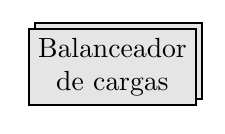
\begin{tikzpicture}
            \node [copy shadow,fill=gray!20,draw=black,thick ,align=center] {Balanceador \\ de cargas};
          \end{tikzpicture}}
        }{}
        \newinst[1]{servico-de-reservas}{\shortstack{Serviço de reservas \\ \\
          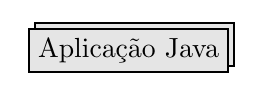
\begin{tikzpicture}
            \node [copy shadow,fill=gray!20,draw=black,thick ,align=center] {Aplicação Java};
          \end{tikzpicture}
        }}{}
        \newinst[1]{banco-de-dados}{\shortstack{Banco de dados \\
          
\begin{tikzpicture}[shape aspect=.5]
            \tikzset{every node/.style={cylinder, shape border rotate=90, draw,fill=gray!25}}
            \node at (1.5,0) {Redis};
          \end{tikzpicture}
        }}{}

        \begin{call}{cliente}{}{api-gateway}{}
          \begin{call}{api-gateway}{}{servico-de-reservas}{}
            \begin{call}{servico-de-reservas}{}{banco-de-dados}{} \end{call}
          \end{call}
        \end{call}
    \end{sequencediagram}
  }
  \caption{Fluxo de reserva de ingressos da aplicação}
  \label{fluxo-de-reserva-de-ingressos-da-aplicacao}
\end{figure}

No contexto da aplicação, cliente web é definido como qualquer consumidor
de API REST (\autoref{rest}) que utilize os dados de um serviço.
O cliente web pode ser um site web, um aplicativo mobile ou até mesmo um serviço
externo que se integra ao sistema de venda de ingressos.

O cliente web conhecerá apenas o endereço do API Gateway (\autoref{api-gateway})
que será responsável por fazer o balanceamento de cargas
(\autoref{balanceador-de-carga}) do serviço de reserva de ingressos.
Toda a regra de negócios referente a reserva de ingressos é executada no
serviço correspondente que possui acesso a um banco de dados (\autoref{banco-de-dados}).
Este responde ao API Gateway que retorna o resultado ao cliente.

Fica abstraído como o cliente é exibido ao usuário
final, possibilitando assim que vários tipos diferentes de clientes implementem
a sua forma de exibição e a própria experiência de visualização para o usuário.
Ou seja, a arquitetura proporciona a clara divisão entre backend
(servidores da aplicação) com frontend (site web, mobile, etc).

Desta arquitetura proposta, a parte prática do trabalho ocorreu apenas na
implementação do serviço de reserva de ingressos (\autoref{implementacao-do-servico}),
deixando o restante apenas como trabalhos futuros (\autoref{trabalhos-futuros}).

\chapter{Implementação do serviço}

Para realizar testes de uma situação real referente às teorias citadas, foi
criado um serviço que registra reservas de ingressos. O serviço possui código
fonte open-source e pode ser acessado em
\url{https://github.com/andreformento/term-paper}.

\section{Código fonte}
Este serviço é uma aplicação escrita na linguagem Java na versão 8. O paradigma
da implementação do código fonte foi Orientação à Objetos. Porém, possui alguns
princípios de programação funcional - como é o caso da técnica de imutabilidade.

\index{alíneas}\index{subalíneas}\index{incisos}Conforme
\cite{does-immutability-really-mean-thread-safety} e \cite{java-doc-immutable-objects},
essa técnica de imutabilidade traz vários benefícios:

\begin{alineas}

  \item Objetos imutáveis facilitam a programação concorrente;

  \item Mudança indesejada em códigos dispersos;

  \item Simplicidade de manutenção do código;

  \item Como a implementação foi em Java, traz benefícios quanto ao algorítimo do
        Garbage Collector.

\end{alineas}

\lstset{language=Java,keywordstyle={\bfseries \color{blue}}}

O primeiro ponto é o mais relevante para a solução, visto que, concorrencia
eficiente é um dos pontos mais importantes. Com a palavra chave \textbf{final} é
possível definir que os atributos da classe não poderão ser alterados depois
de inicializados, conforme exemplo do \autoref{classe-ticket}.

\begin{lstlisting}[label=classe-ticket,caption=Classe Ticket em Java]
public class Ticket implements Serializable {

    @NotNull
    private final String idEvent;

    @NotNull
    private final String idUser;

    @ConstructorProperties({"idEvent", "idUser"})
    public Ticket(String idEvent, String idUser) {
        this.idEvent = idEvent;
        this.idUser = idUser;
    }
    // getters, setters, equals...
}
\end{lstlisting}

\subsection{Spring Boot Framework}

Foi utilizado um framework em Java que possibilita a rápida criação de aplicações.
Conforme \cite[8]{spring-boot-reference-guide}, o Spring Boot Framework torna
produtiva a criação de serviços que rodam de maneira independente, isolada
e com várias opções de acoplar outras bibliotecas que são comuns no desenvolvimento
de software, como integração com banco de dados, sistemas de mensageria, geração
de documentação a partir do código, etc.

%\section{Banco de dados}
%O banco de dados escolhido foi o MongoDB

\subsection{API}

A aplicação desenvolvida gera uma API REST (\autoref{rest}) que é responsável por fazer uma reserva
no evento solicitado. Desta forma, este serviço atende o escopo de reserva de lugar no
evento. Conforme exibido no \autoref{classe-ticket-controller}, existe um endpoint responsável
por fazer essa reserva. Ele tem um contrato que permite que seja informado o evento e
o usuário para realizar a reserva, simplificando a sua utilização.

\index{alíneas}\index{subalíneas}\index{incisos}
Conforme descrito por \cite{mark-richards-software-architecture-patterns},
foi utilizada a arquitetura por camadas para organizar as classes.
A classe \textbf{TicketController} está na camada \textbf{presentation} e tem a
responsabilidade de receber requisições, converter para o padrão utilizado na
aplicação e chamar a classe responsável pela lógica.
Esta classe possui dependência de duas classes:

\begin{alineas}

  \item \textbf{TicketService}

  \begin{alineas}
     \item Fica na camada \textbf{business};
     \item Responsável por lidar com as regras de negócio/lógica do ingresso;
     \item É ela a reponsável por lidar com as validações;
  \end{alineas}

  \item \textbf{TicketMapper}

  \begin{alineas}
     \item Fica na camada \textbf{presentation};
     \item Responsável por converter o que vem de fora da aplicação e transformar
           no padrão adotado dentro da aplicação;
     \item E também o inverso do item anterior: o que for gerado dentro da aplicação -
           seguindo um padrão definido, ela é reponsável por converter
           os dados a serem expostos de modo que mantenha um contrato pré-determinado
  \end{alineas}

\end{alineas}

\begin{lstlisting}[label=classe-ticket-controller,caption=Classe TicketController em Java]
@RestController
@RequestMapping("/events")
public class TicketController {

    private final TicketService service;
    private final TicketMapper mapper;

    public TicketController(TicketService service, TicketMapper mapper) {
        this.service = service;
        this.mapper = mapper;
    }

    @PostMapping
    @RequestMapping("/{idEvent}/tickets")
    public HttpEntity<Resource<TicketResponse>> booking(
        @PathVariable("idEvent") String idEvent,
        @RequestBody final TicketRequest ticketRequest
    ) {

        return mapper.mapToResponse(service.booking(mapper.mapFromRequest(idEvent, ticketRequest)));
    }

}
\end{lstlisting}

\subsection{REST}\label{rest}

\begin{citacao}

REST é um dos modelos de arquitetura que foi descrito por
Roy Fielding \cite[5]{rest-roy-thomas-fielding},
um dos principais criadores do protocolo HTTP, em sua tese de doutorado
e que foi adotado como o modelo a ser utilizado na evolução da arquitetura
do protocolo HTTP.

[...] REST na verdade pode ser considerado como um conjunto de princípios,
que quando aplicados de maneira correta em uma aplicação, a beneficia com a
arquitetura e padrões da própria Web. \cite{rest-principios-e-boas-praticas}.

\end{citacao}

Conforme descrito por \cite{rest-principios-e-boas-praticas}, as aplicações
gerenciam informação que pode ser tratada como recurso. Este recurso que é
gerenciado pela aplicação deve possuir uma identificação única para que seja
possível diferenciar o recurso a ser manipulado em uma requisição.

No protocolo HTTP os recursos podem ser identificados com
URI's (Uniform Resource Identifier) - também conhecido como endpoint.
Desta forma, conforme exibido no \autoref{classe-ticket-controller},
a aplicação criada possui o seguinte endpoint:

% unbreak page não quebra página
% https://tex.stackexchange.com/questions/73231/avoid-page-breaks-in-lstlistings
\begin{minipage}{\linewidth}
\begin{lstlisting}[basicstyle=\ttfamily]
http://localhost:8080/events/\{idEvent\}/tickets
(1)    (2)       (3) (4)     (4)
\end{lstlisting}
\end{minipage}

\index{enumerate}Este endpoint espera uma requisição seguindo o protocolo HTTP
com o método \textbf{POST}, onde cada parte é explicada abaixo:

\begin{enumerate}

  \item Objetos imutáveis facilitam a programação concorrente;

  \item Mudança indesejada em códigos dispersos;

  \item Simplicidade de manutenção do código;

  \item Como a implementação foi em Java, traz benefícios quanto ao algorítimo do
        Garbage Collector.

\end{enumerate}

O seu objetivo é realizar a reserva de um lugar em um determinado evento para um
usuário.

\chapter{Implementação da infraestrutura}\label{implementação-da-infraestrutura}

\section{Ferramentas}\label{ferramentas}

%Motivações (custo) de deixar desacoplarar infraestrutura de software

Há vários serviços que facilitam o desenvolvimento em de aplicações, como banco de dados,
gateways de api, mensageria, etc. Porém, a utilização destes serviços podem
tornar o produto dependente da plataforma onde está rodando. Por isso, é recomendável
a utilização de meios que deixem desacoplados os produtos da plataforma com o produto
digital desenvolvido.

\subsection{Docker}\label{docker}

Foi adotada a ferramenta Docker para que fosse simples a execução do serviço de reserva de ingressos.

\begin{citacao}
O Docker é um conjunto de ferramentas para criar aplicativos distribuídos de forma muito específica.
O foco da filosofia do projeto é a ideia de que os desenvolvedores podem escolher as ferramentas
de que precisam para criar aplicativos da maneira que melhor se adequar às suas necessidades e preferências.
Como resultado, nem todos os projetos usam o Docker da mesma maneira \cite{solomon-hykes}.
\end{citacao}

Conforme descrito por \citeonline{mundodocker-o-que-e-docker}, ``[Docker] facilita a criação e administração de ambientes isolados``.
Ou seja, é uma forma de rodar um aplicação em um ambiente Linux com todos os recursos necessários sem interferir
diretamente na máquina que executa a aplicação - por causa do isolamento.

\begin{citacao}
Contêineres Linux (LXC) é um tipo de
virtualização em nível de sistema operacional que proporciona a execução de múltiplas instâncias isoladas de um determinado
sistema operacional dentro de um único hospedeiro \cite{sinestec-01}.
\end{citacao}

Conforme a citação anterior, é possível executar vários serviços dentro de uma mesma máquina, podendo ser serviços
replicados ou vários tipos diferentes de serviços.
Na aplicação de reserva de ingressos, que foi desenvolvida em Java e precisa de uma JVM para rodar, não precisaria
de nenhuma instalação na máquina de qualquer tipo de programa.
Tudo estaria instalado dentro da imagem Docker criada para rodar a aplicação.
Então, o banco de dados, ou outro serviço que a aplicação dependesse, também poderia rodar em um contêiner Docker.
Ficaria fácil até mesmo trocar toda a implementação para rodar em outra linguagem.

A justificativa para utilizar essa ferramenta também está relacionada a travamentos, rápida execução e desativaçao.
O contêiner é uma evolução em relação ao uso de máquinas virtuais.

\begin{citacao}
Lembrando que cada máquina virtual é um sistema operacional praticamente inteiro instalado sobre um equipamento físico e
rodando para servir a aplicação. Com certeza o servidor de desenvolvimento não teria recursos suficientes para rodar
todos esses sistemas simultaneamente, e nossa máquina física travaria\cite{aprendendo-docker}.
\end{citacao}


Quando se questiona de software, as vantagens da utilização do docker estão em servir como instrumento versátil, que entrega
um ambiente pronto para rodar aplicações. Essa versatilidade pode ser aproveitada para iniciar serviços rapidamente e responder
a aplicação de forma assertiva.


\begin{citacao}
O Docker possibilita o empacotamento de uma aplicação ou ambiente inteiro dentro de um contêiner, e a partir desse momento o
ambiente inteiro torna-se portável para qualquer outro Host que contenha o Docker instalado.
Isso reduz drasticamente o tempo de deploy de alguma infraestrutura ou até mesmo aplicação, pois não há necessidade de ajustes
de ambiente para o correto funcionamento do serviço, o ambiente é sempre o mesmo, configure-o uma vez e replique-o quantas vezes
quiser \cite{mundodocker-o-que-e-docker}.
\end{citacao}

Como mencionado, a redução do tempo é um dos fatores percebidos ao adotar contêineres para execução de aplicações.
A escalabilidade também é satisfeita como descrito na citação abaixo.

\begin{citacao}
Um dos benefícios da abstração entre o sistema host e o contêiner é que, dado um projeto correto de aplicação, a
escalabilidade pode ser simples e direta. Projeto orientado a serviço combinado com aplicações
conteinerizadas fornecem as bases para a escalabilidade fácil.
Um desenvolvedor pode executar alguns contêineres em sua estação de trabalho, enquanto este sistema pode ser escalado
horizontalmente em uma área de preparação ou teste.
Quando os contêineres entram em produção, eles podem escalar novamente
\cite{o-ecossistema-do-docker-uma-visao-geral-da-conteinerizacao-pt}.
\end{citacao}


\subsection{@Kubernetes}\label{kubernetes}

Escrever sobre Kubernetes

\url{https://www.concrete.com.br/2017/06/26/docker-kubernetes-e-openshift/}

\url{https://dzone.com/articles/microservices-with-kubernetes-and-docker}


\section{Requisitos da aplicação}\label{requisitos-da-aplicacao}

Todas as operações mencionadas consideram que o Sistema Operacional é Linux
- que apesar de não ser obrigatório, é recomendado.
Para gerenciamento do código fonte é utilizado o Git no servidor do Github.
Para compilar e rodar a aplicação é necessário ter instalado o Java 8.
Para gerenciamento de pacotes do Java é utilizado o Gradle 4, mas não
é obrigatório que ele esteja instalado - pois é feito o download, caso
ele não exista. Para subir a aplicação é necessário ter o Docker e o
Kubernetes (kubectl e minikube) instalados.

% git, java, gradle, docker, kubernetes

\section{Como rodar a aplicação}\label{como-rodar-a-aplicacao}

Para fazer o download do código fonte é necessário utilizar a ferramenta Git
e executar no terminal do Linux o seguinte mostrado no \autoref{comando-git}.

\lstset{language=bash,keywordstyle={\bfseries \color{black}}}

\begin{lstlisting}[language=bash,label=comando-git,caption=Como fazer o download do código fonte com o Git]
git clone https://github.com/andreformento/term-paper.git
\end{lstlisting}

Para construir a aplicação é necessário executar o comando
\autoref{construir-aplicacao}.

\begin{lstlisting}[language=bash,label=construir-aplicacao,caption=Como construir a aplicação]
cd term-paper
./build.sh
\end{lstlisting}

Para rodar a aplicação é necessário executar o comando
\autoref{rodar-aplicacao}.

\begin{lstlisting}[language=bash,label=rodar-aplicacao,caption=Como rodar a aplicação]
./start.sh
\end{lstlisting}

Para testar a performance da aplicação é necessário executar o comando
\autoref{testar-performance-aplicacao}.

\begin{lstlisting}[language=bash,label=testar-performance-aplicacao,caption=Como testar a performance da aplicação]
./test-report.sh
\end{lstlisting}



% lembrar que o conceito já foi explicado
% só deve ser informado como foram utilizadas as
% ferramentas
% uso do docker para subir a aplicação
% kubernetes para gerenciar o escalamento




\part{Resultados}\label{resultados}
\chapter{Resultados da infraestrutura}
%Foi possível demonstrar uma aplicação que escala sob demanda
%Foi apresentada uma arquitetura que é possível de ser aplicada em produção

\section{Uso da infraestrutura}

A escolha da infraestrutura para a solução final foi o uso da
computação em nuvem (\autoref{infraestrutura-em-nuvem}), visto que, proporciona
escalabilidade que o problema exige - uma das principais vantagens da computação em nuvem.
Além é claro, do baixo custo inicial que a aplicação terá antes de começar a gerar qualquer
tipo de lucro.

Conforme discutido a respeito das topologias das plataformas em
nuvem (\autoref{tipologia-das-plataformas-em-nuvem}), para a solução final foi escolhido o
modelo IaaS (\autoref{iaas}) que fornece a opção de rodar programas como Docker e
Kubernetes, tornando a escolha do serviço de plataforma em nuvem independente da forma
com que o software roda. Ou seja, há um desacoplamento da infraestrutura com o software
(\autoref{ferramentas}).

\section{Análise de desempenho}

Foram feitos vários testes em cima do serviço de reserva de ingressos que foi implementado
(\autoref{implementacao-do-servico}) para saber quais eram seus limites.
É importante deixar claro que a análise ocorrera em um notebook pessoal com poder
de processamento limitado, conforme descrito no
\autoref{anexo-especificacao-de-hardware-do-servidor}.
Em um ambiente real (nuvem \autoref{infraestrutura-em-nuvem})
poderão existir diversas máquinas disponíveis para que sejam utilizadas
(escalabilidade horizontal \autoref{escalabilidade})
permitindo que os números exibidos abaixo sejam muito maiores.

\subsection{Gatling: ferramenta para geração da análise de desempenho}

Os testes de perfomance realizados em cima da aplição de reserva de ingressos foram
feitos com a ferramenta Gatling na versão 2.3.
Com a ferramenta é possível testar alta performance de aplicações web
\cite{gatling-docs} que seguem o protocolo HTTP.

\subsection{Gráficos da análises de desempenhos}

O teste de performance de requisições foi feito usando a
estratégia do método heavisideUsers \cite{gatling-simulation-setup}
que o Gatling possui, simulando assim a utilização simultânea do sistema por
grande quantidade de usuários.
As requisições da análise da
\autoref{03000-requests-config-10s-duration-10},
\autoref{05000-requests-config-10s-duration-10}
e \autoref{10000-requests-config-10s-duration-13}
foram configuradas para serem executadas no período de 10 segundos.
Os testes foram feitos para medir a degradação do sistema em relação ao aumento do
número de requisições simulando um ambiente onde haveriam muitas requisições para
reserva de ingressos.
Com a degração do sistema as respostas começam a demorar mais, ou seja,
o teste demora mais para ser finalizado conforme o aumento do número de requisições.
Com isso, o único parâmetro que muda de um teste para o outro
é o número de requisições realizadas.

Na \autoref{03000-requests-config-10s-duration-10} são feitas 3.000 requisições apenas.
O sistema responde todas elas com sucesso e um desvio padrão de 241 milisegundos
para o tempo de resposta das requisições.
97\% das requisições respondem em menos de 800 milisegundos e apenas 3\% das requisições
respondem em até 1.200 milisegundos.

\begin{figure}[h]
  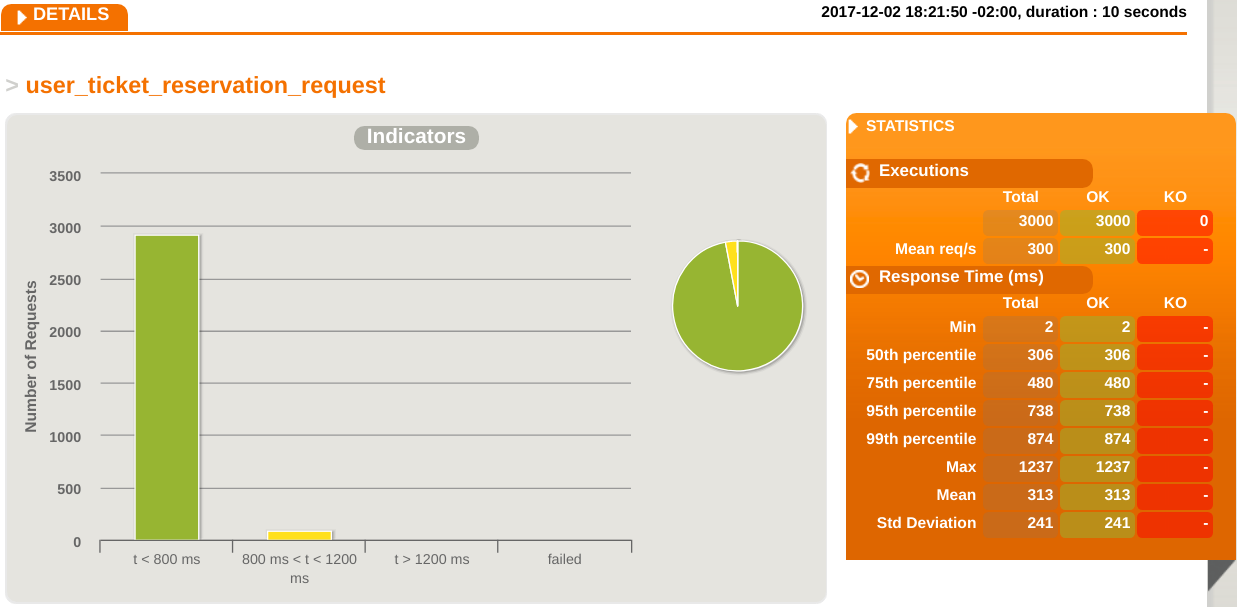
\includegraphics[width=\textwidth]{03000-requests-config-10s-duration-10}
  \caption{Dados do Gatling com 3.000 requisições executados em 10 segundos}
  \label{03000-requests-config-10s-duration-10}
\end{figure}

Na \autoref{05000-requests-config-10s-duration-10} são feitas 5.000 requisições.
O sistema responde todas elas com sucesso e um desvio padrão aumenta para 569 milisegundos
para o tempo de resposta das requisições.
78\% das requisições respondem em menos de 800 milisegundos, 18\% das requisições
respondem em até 1.200 milisegundos e apenas 4\% das requisições
respondem com tempo maior que 1.200 milisegundos.

\begin{figure}[h]
  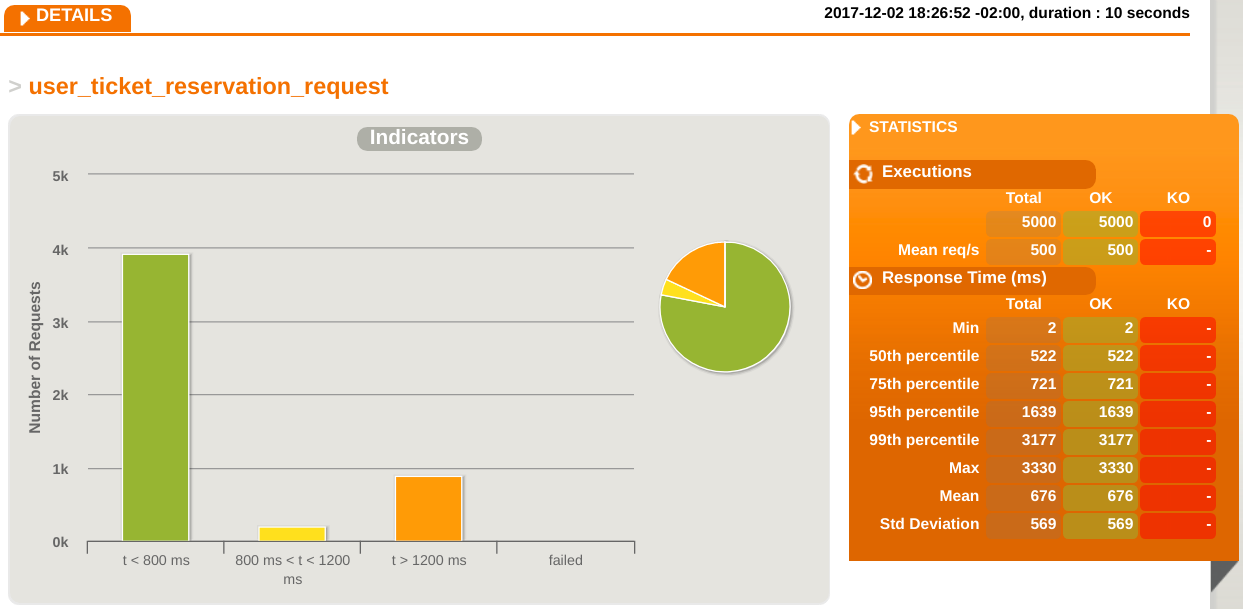
\includegraphics[width=\textwidth]{05000-requests-config-10s-duration-10}
  \caption{Dados do Gatling com 5.000 requisições executados em 10 segundos}
  \label{05000-requests-config-10s-duration-10}
\end{figure}

Na \autoref{10000-requests-config-10s-duration-13} são feitas 10.000 requisições.
O sistema responde todas elas com sucesso e um desvio padrão aumenta para 1117 milisegundos
para o tempo de resposta das requisições.
5\% das requisições respondem em menos de 800 milisegundos, 3\% das requisições
respondem em até 1.200 milisegundos e apenas 93\% das requisições
respondem com tempo maior que 1.200 milisegundos. Aqui fica claro que há grande
degradação do sistema quanto ao tempo de resposta. Porém, o mais importante
é que todas as requisições foram atendidas e o tempo ainda é aceitável para
um ambiente de produção.

\begin{figure}[h]
  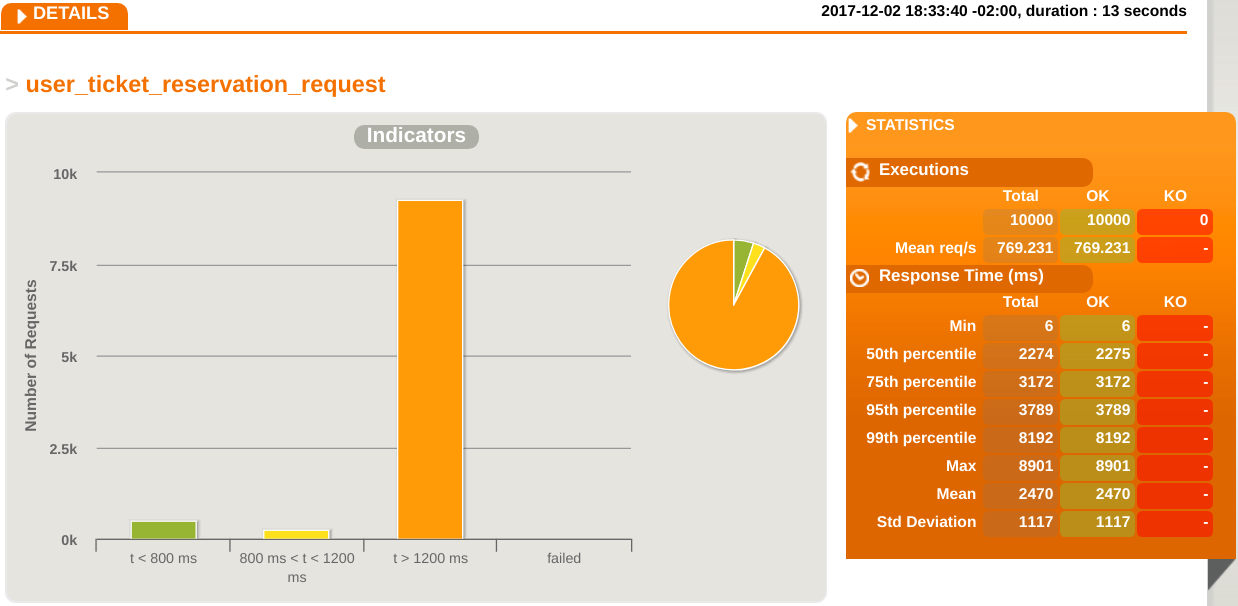
\includegraphics[width=\textwidth]{10000-requests-config-10s-duration-13}
  \caption{Dados do Gatling com 10.000 requisições executados em 13 segundos}
  \label{10000-requests-config-10s-duration-13}
\end{figure}

A \autoref{28000-requests-config-30s-duration-34} possui o tempo de teste configurado
com 30 segundos de execução.
O que se pode concluir com os dados analisados é que a aplicação consegue atender
em torno de 28.000 requests com sucesso em 30 segundos com desvio padrão de
4111 milisegundos.
O tempo de respostas é considerado alto - imaginando um usuário aguardando em
torno de 5 segundos para saber se sua reserva foi realizada.
Porém, a solicitação da reserva é atendida.

Com a escalabilidade horizontal é possível começar a expandir esse poder de processamento.
Com mais máquinas disponíveis o tempo de resposta das aplicações poderia ser reduzido.

\begin{figure}[h]
  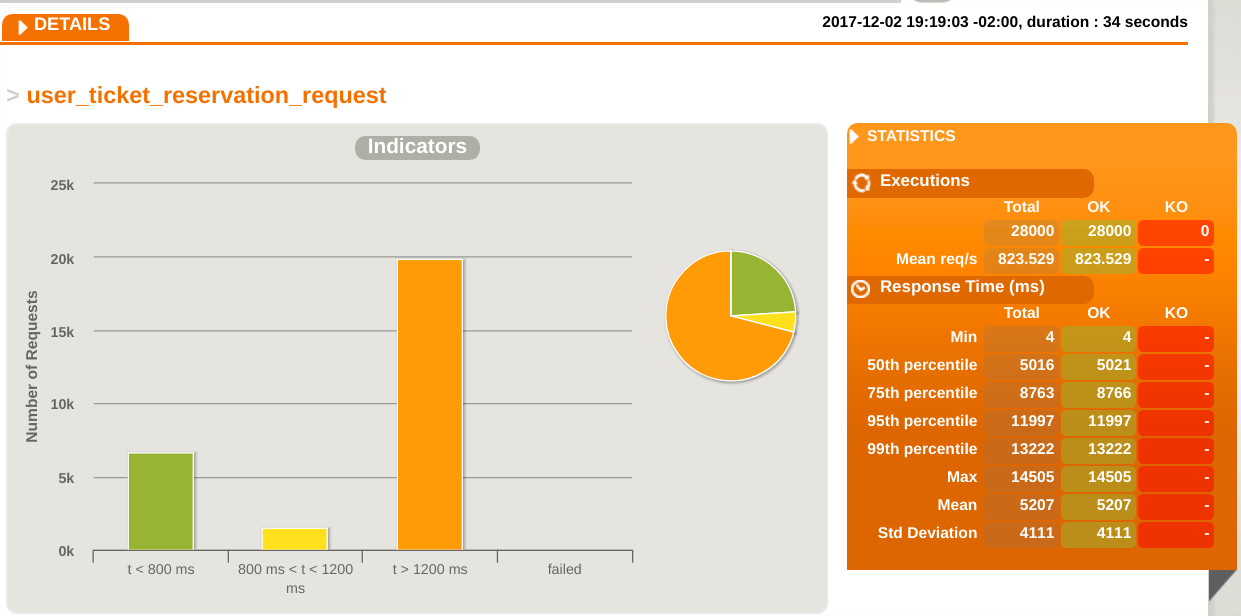
\includegraphics[width=\textwidth]{28000-requests-config-30s-duration-34}
  \caption{Dados do Gatling com 28.000 requisições executados em 34 segundos}
  \label{28000-requests-config-30s-duration-34}
\end{figure}

Todos os resultados com todos os testes realizados pode ser consultados de maneira
iterativa através do link \url{https://andreformento.github.io/term-paper/index.html}.


\chapter*[Conclusão]{Conclusão}
\addcontentsline{toc}{chapter}{Conclusão}

% microserviços
As vantagens que os microseviços trazem foram o motivo da escolha por esta abordagem.
Isso possibilitou separar e implementar apenas uma parte
de uma solução mais geral, que é a venda de ingressos.
Foi possível também que os testes de performance fossem realizados num ponto específico
e deixado claro o comportamento no momento da vendas de ingressos.
Esses dados geram estimativas inclusive para tomadas de decisão quanto aos custos
que uma venda de ingressos pode gerar - e a escolha de qual plataforma utilizar.

% resultados
O resultados apresentados mostram que houve degradação dos serviços com o aumento do
número de requisições.
% escalabilidade / balanceamento de cargas
Porém, usando a abordagem de escalabilidade horizontal e o balanceamento de cargas,
é possível que mais servidores sejam disponibilizados para atender essa alta demanda.

Como o serviço de reserva de ingressos está desacoplado em um serviço de contexto bem
definido, é possível lidar com ele de maneira independente.
% nuvem
Isso em um ambiente de nuvem (IaaS) torna possível a auto escalabilidade com baixo esforço.
Com o uso de ferramentas que auxiliam na implantação, como Docker e Kubernetes,
é possível automatizar o ambiente para que se comporte de maneira otimizada -
quando há grande demanda, vários servidores são disponibilizados, mas no momento
de baixa utilização, várias máquinas podem ser desligadas.
% performance / disponibilidade
Isso influência no desempenho do sistema.
A performance e a disponibilidade é garantida e a degradação é minimizada.

% conclusão final :D
Para o usuário final a experiência de comprar um ingresso em um sistema desses
é positiva, visto que, mesmo que vários outros usuários estão tentando
fazer aquela mesma compra, ele não é afetado e consegue concluir de maneira
satisfatória o processo.

%\chapter{Trabalhos futuros}\label{trabalhos-futuros}

\chapter*[Trabalhos futuros]{Trabalhos futuros}\label{trabalhos-futuros}
\addcontentsline{toc}{chapter}{Trabalhos futuros}

% escrever o serviço em outra linguagem

Em um contexto de um sistema de venda de ingressos, poderiam ser feitos serviços que atendessem
outras necessidades de negócio, como serviço de venda do ingresso, serviço de listagem de eventos
e assim por diante.
Também poderiam ser abordados temas como segurança, controles de acesso e serviço de usuário.

Poderia ser feito um trabalho com uma abordagem diferente para lidar com a venda de ingressos.
Há outras linguagens que lidam com concorrência de maneira mais otimizada,
proporcionando assim uma melhora no tempo de resposta da aplicação com a mesma quantidade
de recursos.
O Whatsapp, por exemplo, utiliza a linguagem Erlang \citeonline{why-whatsapp-used-erlang} que
atende milhares de requisições por segundo.

Há também uma abordagem de microsserviços utilizando o modelo de coreografia, onde seria possível
lidar com o atendimento de muitas requisições de maneira assíncrona, conforme dito por
\cite{scaling-microservices-event-stream}.

Atualmente não é possível que um usuário final faça uma iteração com a aplicação. O desenvolvimento
de uma aplicação frontend, como mobile ou website, poderia explorar o aspecto de usabilidade
do sistema.


% ----------------------------------------------------------
% Referências bibliográficas
% ----------------------------------------------------------
% \nocite{redes-e-servidores}
\nocite{disponibilidade-tolerancia-a-falhas-conceitos-e-exemplos}
\nocite{disponibilidade-avarias-erros-e-falhas}
\nocite{spring-boot-reference-guide}

\bibliography{referencias-bibliograficas}

% ----------------------------------------------------------
% Glossário
% ----------------------------------------------------------
%
% Consulte o manual da classe abntex2 para orientações sobre o glossário.
%
%\glossary

%\begin{apendicesenv}
    
    % Imprime uma página indicando o início dos apêndices
    \partapendices
    
    \chapter{Algum apêndice}
    
    escreve sobre algum apêndice
    
    \chapter{Outro apêndice}

    escreve sobre outro apêndice
    
\end{apendicesenv}


\begin{anexosenv}

    % Imprime uma página indicando o início dos anexos
    \partanexos

    \chapter{Especificação de hardware do servidor}

        \index{alíneas}\index{subalíneas}\index{incisos}As especificações de Hardware
        do computador que foram feitos os testes estão descritas nos próximos tópicos.
        Os testes foram realizados em um notebook de uso pessoal.

        \begin{alineas}

        \item CPU

        \begin{alineas}

            \item Arquitetura: x86\_64

            \item Empresa: Intel Corp.

            \item Produto: Intel(R) Core(TM) i7-4.800MQ CPU @ 2,70GHz

            \item Quantidade de núcleos: 8

            \item Frequência padrão: 2.848MHz

            \item Frequência mínima:  800MHz

            \item Frequência máxima: 3.700MHz

            \item Virtualização: VT-x

            \item L1d cache: 32K

            \item L1i cache: 32K

            \item L2 cache: 256K

            \item L3 cache: 6.144K

        \end{alineas}

        \item Memória

        \begin{alineas}

            \item Capacidade por unidade: 8.192 MB

            \item Quantidade: 2

            \item Capacidade total: 16.384 MB

            \item Modelo: SODIMM

            \item Set: None

            \item Tipo: DDR3

            \item Velocidade: 1.600 MT/s

        \end{alineas}

        \item Armazenamento

        \begin{alineas}

            \item Modelo: Samsung SSD 840

            \item Empresa: Samsung

            \item Device: SSD 840

            \item Detalhe: Samsung SSD 840 PRO Series (DXM05B0Q)

            \item Capacdade: 256 GB

        \end{alineas}

        \item Sistema operacional

        \begin{alineas}

            \item Sistema operacional: Linux

            \item Distro: Fedora

            \item Release: 26

            \item Versão do Kernel: 4.13.12-200.fc26.x86\_64

        \end{alineas}

        \end{alineas}

    %\chapter{Outro anexo}

    %escreve outro anexo

\end{anexosenv}


%---------------------------------------------------------------------
% INDICE REMISSIVO
%---------------------------------------------------------------------
%\phantompart
%\printindex
%---------------------------------------------------------------------

\end{document}
